\documentclass{article}

%% PAQUETES

% Paquetes generales
\usepackage[margin=2cm, paperwidth=210mm, paperheight=297mm]{geometry}
\usepackage[spanish]{babel}
\usepackage[utf8]{inputenc}
\usepackage{gensymb}

% Paquetes para estilos
\usepackage{textcomp}
\usepackage{setspace}
\usepackage{colortbl}
\usepackage{color}
\usepackage{color}
\usepackage{upquote}
\usepackage{xcolor}
\usepackage{listings}
\usepackage{caption}
\usepackage[T1]{fontenc}
\usepackage[scaled]{beramono}

% Paquetes extras
\usepackage{amssymb}
\usepackage{float}
\usepackage{graphicx}
\usepackage{url}
\usepackage[toc,page]{appendix}
\usepackage{mips}


%% Fin PAQUETES


% Definición de preferencias para la impresión de código fuente.
%% Colores
\definecolor{gray99}{gray}{.99}
\definecolor{gray95}{gray}{.95}
\definecolor{gray75}{gray}{.75}
\definecolor{gray50}{gray}{.50}
\definecolor{keywords_blue}{rgb}{0.13,0.13,1}
\definecolor{comments_green}{rgb}{0,0.5,0}
\definecolor{strings_red}{rgb}{0.9,0,0}

%% Caja de código
\DeclareCaptionFont{white}{\color{white}}
\DeclareCaptionFont{style_labelfont}{\color{black}\textbf}
\DeclareCaptionFont{style_textfont}{\it\color{black}}
\DeclareCaptionFormat{listing}{\colorbox{gray95}{\parbox{16.78cm}{#1#2#3}}}
\captionsetup[lstlisting]{format=listing,labelfont=style_labelfont,textfont=style_textfont}

\lstset{
	aboveskip = {1.5\baselineskip},
	backgroundcolor = \color{gray99},
	basicstyle = \ttfamily\footnotesize,
	breakatwhitespace = true,   
	breaklines = true,
	captionpos = t,
	columns = fixed,
	commentstyle = \color{comments_green},
	escapeinside = {\%*}{*)}, 
	extendedchars = true,
	frame = lines,
	keywordstyle = \color{keywords_blue}\bfseries,
	language = C,                       
	numbers = left,
	numbersep = 5pt,
	numberstyle = \tiny\ttfamily\color{gray50},
	prebreak = \raisebox{0ex}[0ex][0ex]{\ensuremath{\hookleftarrow}},
	rulecolor = \color{gray75},
	showspaces = false,
	showstringspaces = false, 
	showtabs = false,
	stepnumber = 1,
	stringstyle = \color{strings_red},                                    
	tabsize = 2,
	title = \null, % Default value: title=\lstname
	upquote = true,                  
}

%% FIGURAS
\captionsetup[figure]{labelfont=bf,textfont=it}
%% TABLAS
\captionsetup[table]{labelfont=bf,textfont=it}

% COMANDOS

%% Titulo de las cajas de código
\renewcommand{\lstlistingname}{Código}
%% Titulo de las figuras
\renewcommand{\figurename}{Figura}
%% Titulo de las tablas
\renewcommand{\tablename}{Tabla}
%% Referencia a los códigos
\newcommand{\refcode}[1]{\textit{Código \ref{#1}}}
%% Referencia a las imagenes
\newcommand{\refimage}[1]{\textit{Imagen \ref{#1}}}

%% APENDICES
\addto\captionsspanish{
	\renewcommand\seename{Apéndices}
	\renewcommand\appendixname{Apéndices}
	\renewcommand\appendixpagename{Apéndices}
}


\begin{document}
\pagenumbering{roman}
\setcounter{page}{5}

% TÍTULO, AUTORES Y FECHA
\begin{titlepage}
	\vspace*{\fill}
	\begin{center}
		\huge{Trabajo Pŕactico N°0} \\
		\medskip
		\Huge \textit{``Infraestructura básica''} \\
		
		\bigskip\bigskip\bigskip\bigskip\bigskip

		\Large Belén Beltran, Padrón Nro. 91.718 \\
		\large \textit{belubeltran@gmail.com} \\ \medskip
		\Large Pablo Ariel Rodriguez, Padrón Nro. 93.970 \\
		\large \textit{prodriguez@fi.uba.ar} \\ \medskip
		\Large Federico Martín Rossi, Padrón Nro. 92.086 \\
		\large \textit{federicomrossi@gmail.com} \\

		\bigskip\bigskip\bigskip\bigskip\bigskip\bigskip\bigskip

		\large 2do. Cuatrimestre 2013 \\ \smallskip
		\large 66.20 Organización de Computadoras \\ \smallskip
		\large Facultad de Ingeniería, Universidad de Buenos Aires \\ \smallskip

		\date{}
	\end{center}
	\vspace*{\fill}
\end{titlepage}

\newpage
\newpage \textit{}
\newpage



% ÍNDICE
\tableofcontents
\newpage \textit{}
\newpage
\pagenumbering{arabic}




% Introducción
\section{Introducción}
	
	En el presente trabajo se tiene como objetivo la familiarización con las herramientas de software que se utilizarán a lo largo de los siguientes trabajos prácticos, llevando a cabo la implementación de un programa que resuelve cierta problemática piloto detallada en los próximos apartados.
	\par
	La implementación se realizará en el lenguaje de programación C. Luego se ejecutará la aplicación sobre una plataforma \textit{NetBSD/MIPS-32} mediante el emulador \textit{GXEmul} \cite{GXEMUL}. Finalmente generaremos, mediante el compilador \textit{GCC} \cite{GCC}, el equivalente en assembler MIPS del código fuente en C.
	\par
	Todos los archivos y códigos fuente aquí mencionados, así como también el presente informe, pueden ser descargados como un archivo comprimido ZIP del repositorio del grupo\footnote{URI del Repositorio: \url{https://github.com/federicomrossi/6620-trabajos-practicos-2C2013/tree/master/tp0}}.
\bigskip




% Compilación
\section{Compilación}
	
	La herramienta para compilar el código en lenguaje C será el \textit{GCC}.
	\par
	Para automatizar las tareas de compilación se hace uso de la herramienta \textit{GNU Make}. Los Makefiles utilizados para la compilación se incluyen junto al resto de los archivos fuentes del presente trabajo.
\bigskip




% Utilización
\section{Utilización}
	
	Veamos ahora la forma en la que debe ser ejecutado el programa implementado en lenguaje C. El resultado de la compilación con ``make'' será un programa ejecutable, de nombre \textit{tp0}, que podrá ser invocado con los siguientes parámetros:
\medskip

\begin{itemize}

\itemsep=2pt \topsep=0pt \partopsep=0pt \parskip=0pt \parsep=0pt
	\item \textit{-h}:  Imprime ayuda para la utilización del programa;
	\item \textit{-V}:  Imprimer la versión actual del programa;
	\item \textit{-r [Width]x[Height]}: Setea la resolución en píxeles del bitmap;
	\item \textit{-o [Path]}: Especifica la ruta del archivo de salida sobre el cual se guarda el tablero generado por la aplicación.

\end{itemize}
\medskip


	Entonces, si se desea generar un tablero con una resolución de 100x100 píxeles sobre el archivo de nombre imagen.pgm, debe ejecutarse el comando de la siguiente manera:
	\bigskip

	{\ttfamily\footnotesize
	\$ ./tp0  -r 100x100 -o imagen.pgm\\}

	En caso de no desear generar un archivo, y solo se espera ver el contenido del archivo por salida estándar, debe ejecutarse el comando de la siguiente manera:
	\bigskip

	{\ttfamily\footnotesize
	\$ ./tp0  -r 100x100 -o -\\}
\medskip




% Implementación
\section{Implementación}
	
	En lo que sigue de la sección, se presentarán los códigos fuente de la implementación del algoritmo. Aquellos lectores interesados en la implementación completa del programa, pueden dirigirse al apéndic ubicado al final del presente informe.
\bigskip



\subsection{Implementación en C}

	La implementación del programa fue divida en los siguientes módulos:
	\medskip

\begin{itemize}

\itemsep=2pt \topsep=0pt \partopsep=0pt \parskip=2pt \parsep=0pt
	\item \textbf{tp0}: Programa principal responsable de interpretar los parámetros especificados a través de la terminal de modo de que realice las tareas solicitadas por el usuario. Su función es, de acuerdo al parámetro o los parámetros especificados, llevar a cabo la ejecución solicitada haciendo uso de módulos externos;
	\item \textbf{pgm}: Módulo encargado de generar una imagen de un tablero de ajedrez (cuadrado, de ocho casilleros de lado) conforme a los parámetros ingresados. Se utiliza para ello el formato gráfico PGM o \textit{portable gray map}. De especificarse un archivo de salida, la imagen en formato PGM se almacenará en este medio.

\end{itemize}	
\bigskip


% Algoritmo PGM
\subsubsection{Algoritmo \textit{Pgm}}

	En el \refcode{codeBSh} se muestra el header de la librería, donde se declara la función \textit{pgm()}, mientras que en el \refcode{codeBSc} se muestra la definición de la librería.

% Código
\lstset{ language = C } % Cambiamos el lenguaje para que parsee en C
\lstinputlisting[label=codeBSh,caption=``pgm.h'']{../codigo/pgm.h} 
\medskip


% Código
\lstset{ language = C } % Cambiamos el lenguaje para que parsee en C
\lstinputlisting[label=codeBSc,caption=``pgm.c'']{../codigo/pgm.c} 
\bigskip\bigskip




\subsection{Generación de código del algoritmo \textit{Pgm} en Assembly MIPS32}

	A continuación se presenta el código en Assembly MIPS32 del algoritmo \textit{Pgm} generado automáticamente por el compilador \textit{GCC}. En el \textit{Apéndice A}	 se encuentra el código del programa en su totalidad.
	\medskip

% Código
\lstset{ language = [mips]Assembler } % Cambiamos el lenguaje para que parsee en MIPS
\lstinputlisting[label=codeBShs,caption=``pgm.s'']{../codigo/pgm.s} 
\bigskip\bigskip



% Debugging
\section{Debugging}
	
	Para analizar el correcto funcionamiento del programa se crearon casos de prueba pertinentes, considerando combinaciones diferentes en el ingreso de parámetros al programa principal, como también tomando en cuenta las diferentes salidas obtenidas a partir del algorirmo \textit{pgm}. Los resultados fueron comparados con los casos esperados y así se determinó el correcto funcionamiento del programa en su totalidad.
\bigskip\bigskip




% Pruebas
\section{Pruebas}

\subsection{Pruebas al ingreso y egreso de datos del programa}
\medskip

	A modo de prueba del programa, se ingresaron ciertos parámetros a éste y se analizó la salida obtenida. A continuación se presentan algunas pruebas realizadas y los resultados obtenidos.
	\par
	El primer caso consiste en crear un tablero de resolución 11x16 y que el resultado sea enviado a la salida estandar. Se debe ingresar por consola lo siguiente:
	\bigskip

{\ttfamily\footnotesize
\indent \$ ./tp0 -r 11x16 -o -\\}
\smallskip

	La salida del programa es la siguiente:
	\bigskip

{\ttfamily\footnotesize
	\indent P2 \\
	\indent \# - \\
	\indent 11 16 \\
	\indent 1 \\
	\indent 1 1 0 0 1 1 0 1 0 1 0 \\
	\indent 1 1 0 0 1 1 0 1 0 1 0 \\
	\indent 0 0 1 1 0 0 1 0 1 0 1 \\ 
	\indent 0 0 1 1 0 0 1 0 1 0 1 \\ 
	\indent 1 1 0 0 1 1 0 1 0 1 0 \\ 
	\indent 1 1 0 0 1 1 0 1 0 1 0 \\ 
	\indent 0 0 1 1 0 0 1 0 1 0 1 \\ 
	\indent 0 0 1 1 0 0 1 0 1 0 1 \\ 
	\indent 1 1 0 0 1 1 0 1 0 1 0 \\ 
	\indent 1 1 0 0 1 1 0 1 0 1 0 \\ 
	\indent 0 0 1 1 0 0 1 0 1 0 1 \\ 
	\indent 0 0 1 1 0 0 1 0 1 0 1 \\ 
	\indent 1 1 0 0 1 1 0 1 0 1 0 \\ 
	\indent 1 1 0 0 1 1 0 1 0 1 0 \\ 
	\indent 0 0 1 1 0 0 1 0 1 0 1 \\ 
	\indent 0 0 1 1 0 0 1 0 1 0 1 \\ 
}
\bigskip


	La segunda prueba consiste en crear un tablero de resolución 16x11 y también enviar la salida a consola. Se debe ingresar por la línea de comandos:
	\bigskip

{\ttfamily\footnotesize
\indent \$ ./tp0 -r 16x11 -o -\\}
\smallskip

	La salida del programa es la siguiente:
	\bigskip

{\ttfamily\footnotesize
	\indent P2 \\
	\indent \# - \\
	\indent 16 11 \\
	\indent 1 \\
	\indent 1 1 0 0 1 1 0 0 1 1 0 0 1 1 0 0 \\
	\indent 1 1 0 0 1 1 0 0 1 1 0 0 1 1 0 0 \\
	\indent 0 0 1 1 0 0 1 1 0 0 1 1 0 0 1 1 \\
	\indent 0 0 1 1 0 0 1 1 0 0 1 1 0 0 1 1 \\
	\indent 1 1 0 0 1 1 0 0 1 1 0 0 1 1 0 0 \\
	\indent 1 1 0 0 1 1 0 0 1 1 0 0 1 1 0 0 \\
	\indent 0 0 1 1 0 0 1 1 0 0 1 1 0 0 1 1 \\
	\indent 1 1 0 0 1 1 0 0 1 1 0 0 1 1 0 0 \\
	\indent 0 0 1 1 0 0 1 1 0 0 1 1 0 0 1 1 \\
	\indent 1 1 0 0 1 1 0 0 1 1 0 0 1 1 0 0 \\
	\indent 0 0 1 1 0 0 1 1 0 0 1 1 0 0 1 1 \\
}
\bigskip


	La tercer prueba consiste en generar el tablero de tamaño default 8x8 (se genera en caso de no ingresar la opción -r), ingresando por consola:
	\bigskip

{\ttfamily\footnotesize
\indent \$ ./tp0 -o -\\}
\smallskip

	El resultado del programa se ve por salida standard y es el siguiente:
	\bigskip

{\ttfamily\footnotesize
	\indent P2 \\
	\indent \# - \\
	\indent 8 8 \\
	\indent 1 \\
	\indent 1 0 1 0 1 0 1 0 \\
	\indent 0 1 0 1 0 1 0 1 \\
	\indent 1 0 1 0 1 0 1 0 \\
	\indent 0 1 0 1 0 1 0 1 \\
	\indent 1 0 1 0 1 0 1 0 \\
	\indent 0 1 0 1 0 1 0 1 \\
	\indent 1 0 1 0 1 0 1 0 \\
	\indent 0 1 0 1 0 1 0 1 \\
}
\bigskip


	Una prueba más interesante, es aquella en la cual la resolución permite ver una imagen bastante amplia. En este caso se considera una resolución de 200x200 y se decide guardar la salida en un archivo. Se debe ingresar por consola:
	\bigskip

{\ttfamily\footnotesize
\indent \$ ./tp0 -r 200x200 -o 200x200.pgm\\}
\smallskip

	La salida en formato de imagen \textit{PGM} se muestra en la \textit{Figura 1}.


\newpage
\begin{figure}[H]
	\centering
	
\includegraphics[width=0.36\textwidth]{images/200x200.jpg}
	\medskip
	\caption{Imágen del tablero de ajedrez con resolución de 200x200 píxeles.}
\end{figure}
\bigskip\bigskip


\subsection{Tiempos de ejecución}

	\par
	Se quiere medir el tiempo que tarda el programa en la máquina virtual MIPS32 en crear un tablero de ajedrez con ciertas características. Para ello se realizó un módulo aparte que, con la ayuda del comando \textit{GNU ``time''} \cite{TIME}, mide los tiempos de la realización de un tablero de resolución 1x1 hasta uno de 1000x1000. 
	\par
	Los datos obtenidos se pueden observar en el \textit{Cuadro 1}. 
	\bigskip\bigskip


% Tabla 1
\begin{table}[!hbt]
	\begin{center}
	\begin{tabular}{|>{\centering\arraybackslash}m{3cm}|>{\centering \arraybackslash}m{3cm}|}
		\hline
		\rowcolor[gray]{0.9}\textbf{Resolución} & \textbf{Tiempo de ejecución [s]}\\
		\hline
		\centering 1x1 & 0,051 \\
		\hline
		\centering 100x100 & 0,316 \\
		\hline
		\centering 200x200 & 1,148 \\
		\hline
		\centering 300x300 & 2,5 \\
		\hline
		\centering 400x400 & 4,434 \\
		\hline
		\centering 500x500 & 6,844 \\
		\hline
		\centering 600x600 & 9,848 \\
		\hline
		\centering 700x700 & 13,5 \\
		\hline
		\centering 800x800 & 17,449 \\
		\hline
		\centering 900x900 & 22,152 \\
		\hline
		\centering 1000x1000 & 27,613 \\
		\hline
	\end{tabular}
	\smallskip
	\caption{Tiempos en segundos obtenidos en la ejecución\\ del programa para distintas resoluciones.}
	\end{center}
\end{table}
\bigskip\bigskip


	En la \textit{Figura 2} se presenta un diagrama resumido de los tiempos de ejecución obtenidos. Como es de esperar, se obtiene una curva cuadrática.


\newpage	
% Figura 2
\begin{figure}[h]
	\centering
	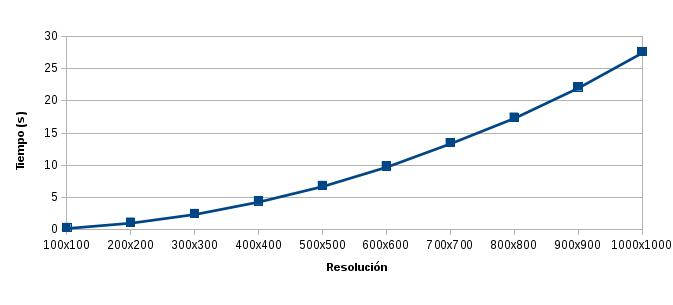
\includegraphics[width=1.0\textwidth]{images/grafico-tiempos.jpg}
	\caption{Gráfico de tiempo de ejecución (en segundos) respecto\\ de la resolución de imagen generada.}
\end{figure}
\bigskip\bigskip\bigskip




% Citas bibliográficas.
\begin{thebibliography}{99}

	\bibitem{GXEMUL} The NetBSD project, \url{http://www.netbsd.org/}

	\bibitem{GCC} GCC, the GNU Compiler Collection, \url{http://gcc.gnu.org/}

	\bibitem{BS} PGM format speciffication, \url{http://netpbm.sourceforge.net/doc/pgm.html}

	\bibitem{TIME} time man page, \url{http://unixhelp.ed.ac.uk/CGI/man-cgi?time}

	\bibitem{HEN00} J. L. Hennessy and D. A. Patterson, ``Computer Architecture. A Quantitative
	Approach,'' 4th Edition, Morgan Kaufmann Publishers, 2000.

	\end{thebibliography}

\newpage


% Apendices
\begin{appendices}

\bigskip\bigskip

% Implementación completa en lenguaje C
\section{Implementación completa en lenguaje C}


\subsection{\textit{tp0.c}. Implementación del main del programa}
% Código
\lstset{ language = C } % Cambiamos el lenguaje para que parsee en C
\lstinputlisting[label=codeTP0cfull,caption=``tp0.c'']{../codigo/tp0.c} 
\bigskip\bigskip

\subsection{\textit{pgm.h}. Declaración de la librería Pgm}
% Código
\lstset{ language = C } % Cambiamos el lenguaje para que parsee en C
\lstinputlisting[label=codeBShfull,caption=``pgm.h'']{../codigo/pgm.h} 
\bigskip\bigskip

\subsection{\textit{pgm.c}. Definición de la librería Pgm}
% Código
\lstset{ language = C } % Cambiamos el lenguaje para que parsee en C
\lstinputlisting[label=codeBScfull,caption=``pgm.c'']{../codigo/pgm.c} 
\bigskip\bigskip



% Implementación completa en assembly MIPS
\section{Generación del código completo en assembly MIPS}


\subsection{\textit{tp0.s}. Generación del main del programa}
% Código
\lstset{ language = [mips]Assembler } % Cambiamos el lenguaje para que parsee en C
\lstinputlisting[label=codeTP0afull,caption=``tp0.s'']{../codigo/tp0.s} 
\bigskip\bigskip

\subsection{\textit{pgm.s}. Generación del algoritmo Pgm}
% Código
\lstset{ language = [mips]Assembler} % Cambiamos el lenguaje para que parsee en MIPS
\lstinputlisting[label=codeSSafull,caption=``pgm.s'']{../codigo/pgm.s} 
\bigskip\bigskip


\end{appendices}

\end{document}
